\documentclass[tikz]{standalone}

\begin{document}
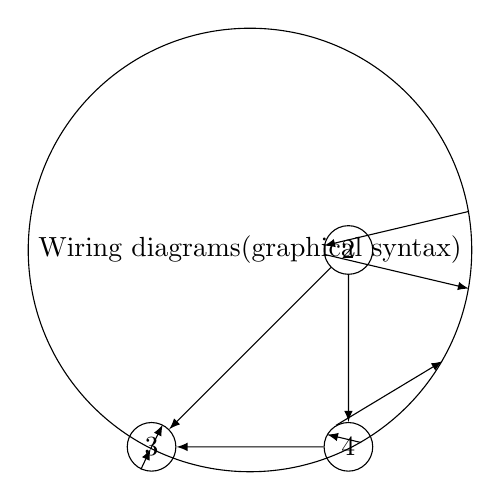
\begin{tikzpicture}[scale=1.25]
\tikzset{vertex/.style = {shape=circle,draw,minimum size=1.5em}}

  \tikzset{edge/.style = {->,> = latex}}

  % vertices

  \node[vertex] (1) at  (1,0) {Wiring diagrams\n(graphical syntax)};

  \node[vertex] (2) at  (2,0) {$2$};

  \node[vertex] (3) at  (0,-2) {$3$};

  \node[vertex] (4) at  (2,-2) {$4$};

  % edges

  \draw[edge] (1.10) to (2.170);

  \draw[edge] (2.190) to (1.350);



  \draw[edge] (1) to (3);

  \draw[edge] (1.300) to (4.150);

  \draw[edge] (2) to (3);

  \draw[edge] (2) to (4);

  \draw[edge] (3) to (1);

  \draw[edge] (4) to (3);

  \draw[edge] (4.120) to (1.330);
\end{tikzpicture}

\end{document}
